\documentclass[11pt,a4paper]{article}

% -------------------------------------------------
% PACKAGES
% -------------------------------------------------
\usepackage[spanish]{babel}
\usepackage[utf8]{inputenc}
\usepackage[T1]{fontenc}
\usepackage{lmodern}
\usepackage[margin=1in]{geometry}

\usepackage{graphicx}
\graphicspath{{./figures/}}
\usepackage{amsmath,amssymb}
\usepackage{booktabs}
\usepackage{xcolor}
\usepackage{hyperref}
\usepackage{fancyhdr}
\usepackage{titlesec}
\usepackage{enumitem}
\usepackage[style=ieee,backend=biber]{biblatex}

\addbibresource{references.bib}

\setlist{
    noitemsep,
    topsep=0pt
}

% -------------------------------------------------
% COLORS
% -------------------------------------------------
\definecolor{primary}{RGB}{25,55,109}

% -------------------------------------------------
% HEADER
% -------------------------------------------------
\pagestyle{fancy}
\fancyhf{}
\fancyhead[L]{Videovigilancia con Interpretación de Escenas}
\fancyfoot[C]{\thepage}

% -------------------------------------------------
% SECTION STYLE
% -------------------------------------------------
\titleformat{\section}
{\large\bfseries\color{primary}}
{\thesection.}{0.5em}{}

% -------------------------------------------------
% DOCUMENT
% -------------------------------------------------
\begin{document}

% =================================================
% TITLE (FULL WIDTH)
% =================================================

\begin{center}

    \vspace{1cm}

    {\Huge\bfseries\color{primary}
        Videovigilancia con Interpretación de Escenas\par}

    \vspace{0.5cm}

    {\Large Analítica de video para seguridad perimetral\par}

    \vspace{0.5cm}

    \large
    \textbf{Autor:} Roberto García Guzmán\\
    \textbf{Institución:} Universidad de Guanajuato\\
    \textbf{Fecha:} \today

    \vspace{0.5cm}

    \rule{0.8\textwidth}{0.5pt}

    \vspace{0.5cm}

\end{center}

\tableofcontents
\newpage

% =================================================
\section{Resumen ejecutivo}


This section introduces the problem context, objectives, and motivation.
You can discuss background information and explain why the topic is relevant.

Lorem ipsum dolor sit amet, consectetur adipiscing elit. Sed do eiusmod tempor
incididunt ut labore et dolore magna aliqua.

% =================================================
\section{Planteamiento del problema}

La seguridad perimetral es un aspecto crítico en la protección de instalaciones, infraestructuras y áreas sensibles. Usualmente incluye elementos como barreras físicas y sistemas electrónicos diseñados para prevenir accesos no autorizados.

Una de las herramientas más efectivas para la protección perimetral es la videovigilancia, que permite monitorear áreas extensas y detectar actividades sospechosas en tiempo real. Sin embargo, si se desea prevenir eventos de seguridad, es necesario contar con un equipo de personas que monitoreen constantemente las cámaras, lo cual puede ser costoso y propenso a errores humanos.

Con el fin de aliviar este inconveniente, se deben implementar sistemas de videovigilancia inteligentes que puedan interpretar las escenas y detectar actividades sospechosas de manera autónoma, alertando a los operadores solo cuando sea necesario.

Bajo este contexto, el objetivo de este proyecto es desarrollar un sistema de videovigilancia autónomo, que tenga la capacidad de interpretar escenas, utilizando técnicas avanzadas de análisis de video e inteligencia artificial.

\subsection{Inteligencia artificial en el análisis de video}

Una de las principales aplicaciones de la inteligencia artificial en el análisis de video en general es la detección de objetos. Esto se refiere a la capacidad de identificar y localizar objetos específicos dentro de una imagen, como personas, vehículos o animales. Esto se hace a través de algoritmos de aprendizaje profundo, como las redes neuronales convolucionales (CNN), que pueden aprender a reconocer patrones visuales complejos.

Este proyecto utiliza una red neuronal convolucional para la detección de objetos relevantes en cada cuadro del video. Una vez detectados estos objetos, se aplica un algoritmo de seguimiento para mantener un registro del movimiento de cada objeto a lo largo del tiempo. Esto permite analizar el comportamiento de los objetos y detectar actividades sospechosas, como intrusión, merodeo o abandono de objetos. Además, se emplea la capacidad de detección de objetos para identificar la presencia de armas de fuego en las escenas.

\subsection{Objetivos}

\begin{itemize}
    \item Desarrollar un algoritmo de análisis de video capaz de detectar cuatro tipos de actividades sospechosas: intrusión, merodeo, abandono de objetos y armas de fuego.
    \item Desarrollar una aplicación web por medio de la cual un usuario pueda configurar el sistema y recibir alertas en tiempo real.
    \item Evaluar el sistema utilizando un conjunto de datos de videovigilancia desde diferentes ángulos y grados de ilumniación.Medir su precisión, tasa de falsos positivos, tiempo de respuesta y recursos computacionales utilizados.
\end{itemize}

\section{Arquitectura del sistema}

\begin{figure}[h!]
    \centering
    
\includegraphics[width=\linewidth]{general_schema.pdf}
    \caption{Arquitectura general del sistema de videovigilancia con interpretación de escenas.}
    \label{fig:general_schema}
\end{figure}

El sistema tiene tres componentes principales: el módulo de detección de objetos, el módulo de seguimiento de objetos y el módulo de análisis de la escena. Estos tres componentes procesan la información como se muestra en el diagrama de la figura \ref{fig:general_schema}.

\subsection{Módulo de detección de objetos}

Detectar un objeto en una imagen consiste en obtener sus coordenadas y dimensiones, en pixeles, dentro de la misma. Se obtiene lo que se conoce como cajas de detección: posición en $x$, posición en $y$, ancho y alto. Usualmente, esta detección va acompañada de una clase, que indica el tipo de objeto del que se trata, y un porcentaje de confianza de que la detección es correcta. Un ejemplo de detección se muestra en la figura \ref{fig:detection}.

\begin{figure}[h!]
    \centering
    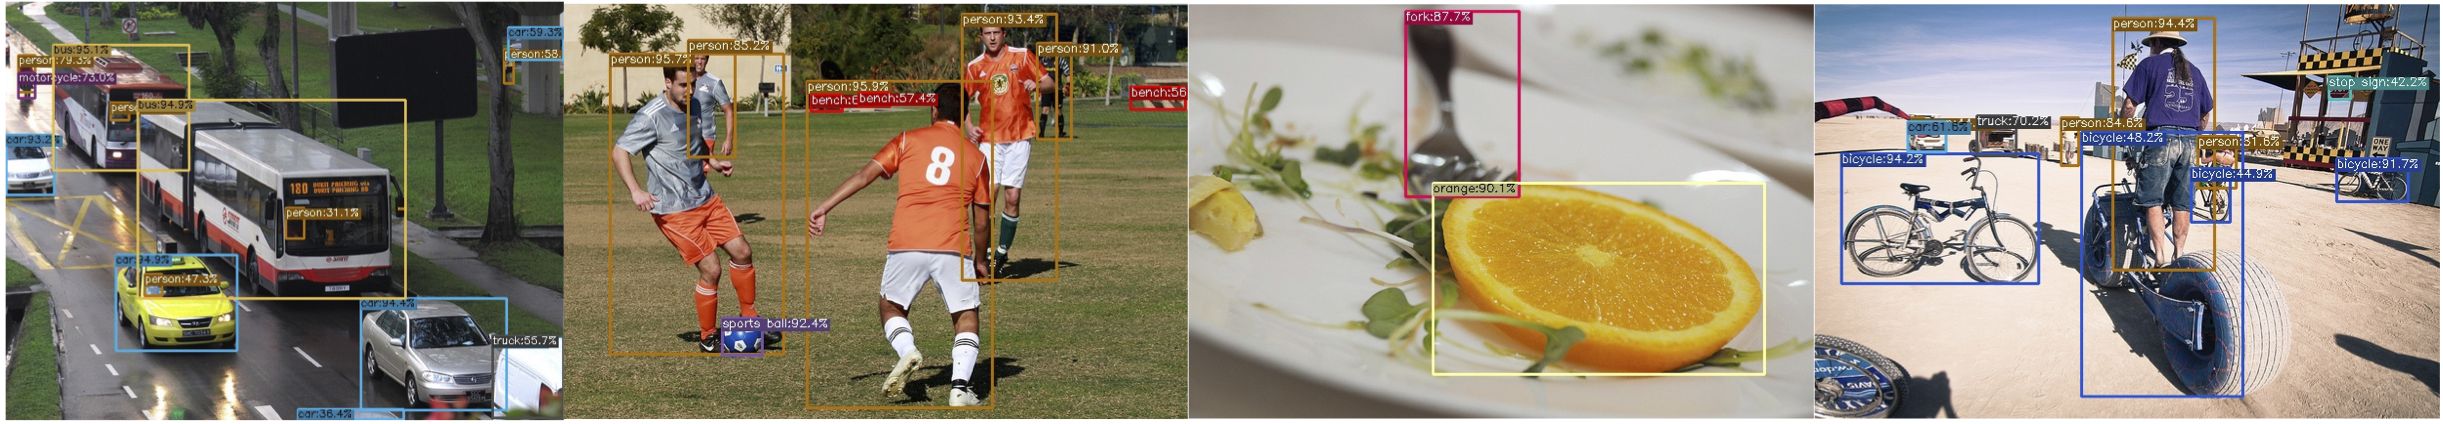
\includegraphics[width=0.9\linewidth]{demo.png}
    \caption{Ejemplo de detección en imágenes en conjunto de datos COCO 2017. Imagen extraída de \url{https://github.com/megvii-basedetection/yolox}.}
    \label{fig:detection}
\end{figure}

Para realizar la detección de los objetos, el módulo de detección emplea el modelo convolucional YOLOX /CITA/, el cual es una mejora de los modelos YOLOv3-v5. Además, tiene la ventaja de que es distribuido bajo la licencia Apache 2.0\footnote{\url{https://github.com/megvii-basedetection/yolox?tab=Apache-2.0-1-ov-file\#readme}} que permite su uso comercial sin restricciones, a diferencia de los modelos YOLOv5 en adelante, que tienen licencia AGPL 3.0\footnote{\url{https://www.ultralytics.com/legal/agpl-3-0-software-license}} que permiten el uso libre solamente para otros proyectos de código abierto.

El modelo YOLOX es capaz de detectar objetos con un bajo costo computacional y en tiempo real. Su arquitectura se muestra en la figura \ref{fig:yolox}, la cual consiste de múltiples capas convolucionales y tres salidas: clase, caja de detección y porcentaje de confianza, referido en este caso como IoU.

\begin{figure}[h!]
    \centering
    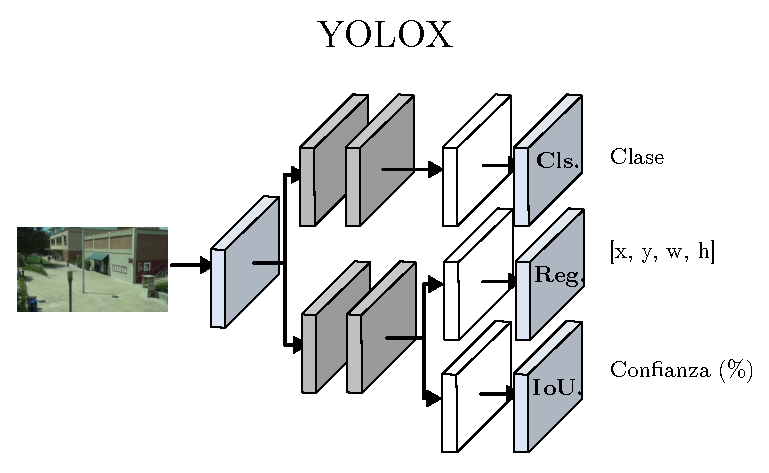
\includegraphics[width=0.6\linewidth]{yolox.pdf}
    \caption{Arquitectura de modelo YOLOX.}
    \label{fig:yolox}
\end{figure}

Este proyecto utiliza un modelo YOLOX pre-entrenado en el conjunto de datos COCO 2017 /CITE/\footnote{\url{https://cocodataset.org/\#download}}. Este conjunto de datos contiene muestras de detección de 80 clases de objetos diferentes. Para este proyecto, se hace una reducción a 4 clases sin modificar la estructura del modelo: personas, vehículos, vehículos ligeros y bolsas. Esta reducción se realiza mediante el mapeo de clases descrito a continuación:

\begin{itemize}
    \item Personas: Personas
    \item Vehículos: Automovil, Autobus, Avión, Tren, Camión, Bote
    \item Vehículos ligeros: Bicicleta, Motocicleta
    \item Bolsas: Mochila, Bolsa de mano, Maleta
\end{itemize}

Las detecciones que no estén en esas categorías son ignoradas, pues corresponden a objetos de bajo interés como comida, animales, mobiliario, etc.

El modelo YOLOX tiene variantes tanto para el tamaño de la imagen de entrada, como del número de capas y parámetros. El modelo que se emplea en este proyecto es el modelo YOLOX\_s (small), el cual procesa imágenes de 640x640 pixeles y tiene 9 millones de parámetros. Con él se alcanza un balance adecuado entre tiempo de respuesta, recursos utilizados y exactitud de la detección.

Adicionalmente, el proyecto requiere detectar objetos como armas de fuego, los cuales no están incluidos en el conjunto de entrenamiento de COCO 2017. Para detectar estos objetos se reentrenó otro modelo YOLOX\_s, en el conjuto de datos de detección de armas Simuletic Synthetic CCTV Weapon-Detection Dataset /CITE/. De este modelo solo se obtienen detecciones de la clase \textit{Arma}.

El módulo de detección de objetos utiliza ambos modelos sobre cada cuadro del video y combina las detecciones como se muestra en la figura \ref{fig:two_yolox}. En total se detectan 5 clases diferentes: personas, vehículos, vehículos ligeros, bolsas y armas de fuego.

\begin{figure}[h!]
    \centering
    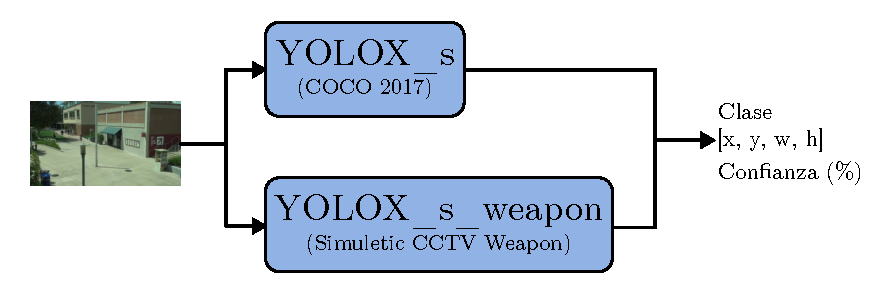
\includegraphics[width=0.7\linewidth]{two_yolox.pdf}
    \caption{Combinación de dos modelos de detección YOLOX\_s.}
    \label{fig:two_yolox}
\end{figure}

\subsection{Módulo de seguimiento de objetos}

El módulo de seguimiento de objetos se encarga de mantener un registro de los objetos detectados a lo largo del tiempo, asignándoles un identificador único. Esto permite analizar el comportamiento de los objetos y detectar actividades sospechosas, como intrusión, merodeo o abandono de objetos. Para realizar el seguimiento de los objetos, se emplea el algoritmo Deep SORT /CITE/, el cual combina la información de las cajas de detección con características visuales extraídas por una red neuronal para mantener un seguimiento robusto incluso en situaciones de oclusión.

El algoritmo Deep SORT utiliza como entrada las cajas de detección obtenidas del módulo de detección de objetos. Con cada caja, extrae el recorte correspondiente de la imagen original y obtiene un vector de características (o descriptor de apariencia), empleando una red neuronal convolucional. Posteriormente, genera un vector de estado que incluye: posición en $x$, posición en $y$, relación de aspecto $a$, altura $h$, velocidad en $x$, velocidad en $y$, cambio de la relación de aspecto $a$ y cambio de altura $h$. Con esta información aplica un filtro de Kalman para predecir el estado del objeto en la siguiente imagen. Finalmente, utiliza el algoritmo húngaro para emparejar las nuevas detecciones con las de la imagen anterior, utilizando tanto la predicción de estado como el descriptor de apariencia. Este algoritmo se ilustra en la figura \ref{fig:deepsort}.

\begin{figure}[h!]
    \centering
    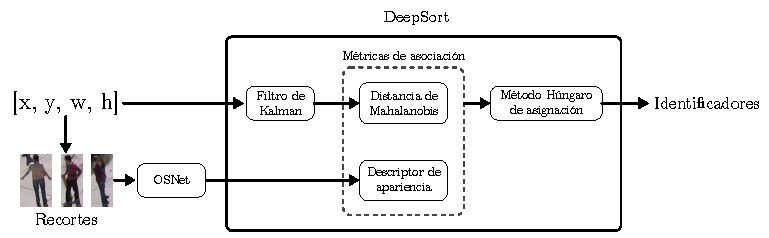
\includegraphics[width=0.9\linewidth]{deepsort.pdf}
    \caption{Algoritmo Deep SORT.}
    \label{fig:deepsort}
\end{figure}

Para generar los descriptores de apariencia, se emplea la la red neuronal convolucional OSNet (Omni-Scale Network) /CITE/, la cual fue diseñada para realizar re-identificación de personas. Esta tarea requiere encontrar características discriminativas que pudan distinguir individuos entre diferentes ángulos de la cámara, lo cual es ideal para un sistema de videovigilancia.

\subsection{Módulo de análisis de la escena}

Este módulo es el encargado de verificar las posiciones de los objetos y emitir las alarmas cuando se presenten eventos de seguridad.

Los cuatro eventos de seguridad son: Intrusión, merodeo, objetos abandonados y armas. A continuación se explica cómo se detecta cada uno de ellos.

\subsubsection{Intrusión}

El proceso de detección de intrusión se ilustra en la figura \ref{fig:intrusion}. Se comienza por generar un polígono que delimita el área restringida, de este polígono se obtiene una máscara del área restringida. Cuando se detecta una persona en la escena, se obtiene su caja de detección y se genera una máscara de detección. Una vez obtenidas ambas máscaras se calcula el área de intersección entre ambs máscaras y se calcula el porcentaje de intrusión como se muestra en la ecuación \ref{eq:perc_intrusion}. Si el porcentaje de intrusión supera el porcentaje mínimo establecido, se emite la alarma.

\begin{equation}\label{eq:perc_intrusion}
    \text{\% Intrusion} = \frac{\text{Area intersección}}{\text{Area detección}}
\end{equation}

Los parámetros que el usuario puede modificar son:

\begin{itemize}
    \item Porcentaje mínimo de intrusión $[0, 100]$
\end{itemize}

\begin{figure}[h!]
    \centering
    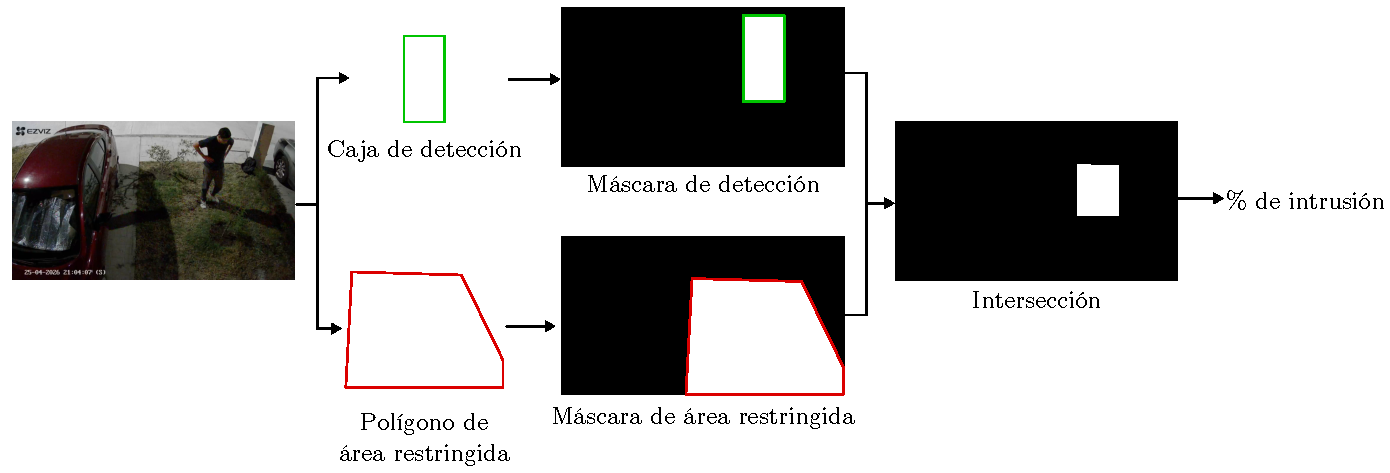
\includegraphics[width=0.9\linewidth]{intrusion.pdf}
    \caption{Algoritmo de detección de intrusiones.}
    \label{fig:intrusion}
\end{figure}

\subsubsection{Merodeo}

A cada objeto en la escena se le asigna un contador que indica el tiempo que ha estado presente. Para ello, cada vez que el objeto es nuevamente detectado, se calcula el tiempo transcurrido entre el cuadro anterior y el actual, y se le suma esa cantidad al contador de tiempo.

Cada cuadro, se verifica el contador de tiempo y si excede el límite de tiempo establecido se emite la alarma.

Los parámetros que el usuario puede modificar son:

\begin{itemize}
    \item Tiempo máximo en escena $[0, \infty)$
\end{itemize}

Es importante destacar que cuando se procesa un video pregrabado, el tiempo entre cuadros no coincide con el tiempo real. Ejemplo: si un video se grabó a 30 FPS, pero se procesa a 5 FPS, el sistema detecta que la duración de un cuadro es de 0.2 segundos, en lugar de 0.033; si se configura un tiempo máximo en escena de 10 segundos, la alarma se activará a los 50 cuadros, en lugar de a los 300. Este comportamiento no sucede en el sistema final, ya que el sistema ignora todos los cuadros intermedios y solamente procesa el cuadro actual.

\subsubsection{Objetos abandonados}

Adicional al tiempo en escena, para cada objeto se almacena su posición una vez cada segundo, durante los últimos N segundos (por defecto 3600). Para detectar un objeto como abandonado, se establece un tiempo máximo en escena, cuando se supera el límiete, se calcula la distancia promedio recorrida por el objeto durante los últimos N segundos y, si esta distancia es cercana a 0, se considera como objeto abandonado.

Los parámetros que el usuario puede modificar son:

\begin{itemize}
    \item Tiempo máximo en escena $[0, \infty)$
\end{itemize}

Sin embargo, se encontró que el modelo YOLOX\_s es deficiente en la detección de objetos como bolsas o mochilas en imágenes CCTV, principalmente debido a que estos objetos se muestranson muy pequeños en las imágenes. Sin la detección de estos objetos, la detección de objetos abandonados no es posible, es por ello que se implementó una estrategia alternativa de detección de objetos desconocidos.

Bajo esta estrategia, se debe obtener el fondo de la escena siguiendo la estrategia ejemplificada en la figura \ref{fig:abandoned_obj_background}. Para ello, se comienza por almacenar los primeros N cuadros del video o la captura en tiempo real, a continuación, los cuadros se convierten a escala de grises y, finalmente, se calcula la mediana de cada pixel para obtener una imagen del fondo.

\begin{figure}[h!]
    \centering
    \includegraphics[width=0.9\linewidth]{abandoned_obj.pdf}
    \caption{Algoritmo de obtención de fondo.}
    \label{fig:abandoned_obj_background}
\end{figure}

Posteriormente, cada cuadro nuevo se convierte a escala de grises y se calcula la diferencia absoluta entre el cuadro y el fondo, dando como resultado una imagen de ``resta'' o diferencia. A esta imagen de diferencia se le aplica un umbral para posteriormente obtiener las regiones (llamadas contornos en OpenCV) que difieren, cada contorno es un posible objeto. Se descartan los contornos que coincidan con algún objeto detectado por el modelo YOLOX\_s y los contornos faltantes se consideran como objetos con clase ``desconocida''. Este proceso se ilustra en la figura \ref{fig:abandoned_obj_unknown}

Los detecciones con clase desconocida se agregan a la lista de detecciones de los modelos YOLOx\_s, para dar un total de 6 clases: persona, vehículo, vehículo ligero, bolsa, desconocido. Solamente los objetos de las clases bolsa y desconocido son considerados para la detección de objetos abandonados.

\begin{figure}[h!]
    \centering
    \includegraphics[width=0.9\linewidth]{abandoned_obj_2.pdf}
    \caption{Algoritmo de detección de objetos desconocidos.}
    \label{fig:abandoned_obj_unknown}
\end{figure}

\subsubsection{Armas de fuego}

La detección de armas de fuego se realiza con el modelo reentrenado YOLOX\_s\_weapon. Para evitar falsos positivos se establce un mínimo de tiempo que el arma debe estar en la escena para que pueda emitirse la alarma. Usualmente, este tiempo es de pocos segundos, por defecto 5.


Los parámetros que el usuario puede modificar son:

\begin{itemize}
    \item Tiempo mínimo en escena $[0, \infty)$
\end{itemize}

\section{Contenido del repositorio}

En respositorio de la aplicación se encuentra dividido en diferentes carpetas correspondientes a paquetes de Python, modelos preentrenados y otros ejemplos.

\begin{itemize}
    \item \textbf{yolox\footnote{Versión original: \url{https://github.com/megvii-basedetection/yolox}}:} Paquete para detección de objetos con el modelo YOLOX. Modificado para adaptalo a la versión de Python y al conjunto de datos de armas para entrenamiento.
    \item \textbf{deepsort\footnote{Version original: \url{https://github.com/kadirnar/deepsort-pip}}:} Paquete para el seguimiento de múltiples objetos en video. Modificado para adaptarlo a la versión de Python y con adiciones para que se integre con el proyecto.
    \item \textbf{yolotracker:} Paquete propio que incluye la lógica de la detección de eventos y combina yolox con deepsort. Este paquete contiene los algoritmos descritos en la sección anterior. Contiene un script para probar el algoritmo en videos pregrabados.
    \item \textbf{video-surveillance-app:} Directorio que contiene la aplicación web para configuración del sistema, así como el servicio que hace la detección de los eventos en tiempo real.
\end{itemize}

\section{Instalación}

La siguiente guía fue probada en una computadora con Windows 10 y Kubuntu 24.04. El hardware es Intel Core i5-10300H, NVIDIA GeForce GTX 1050 Ti (4 GB), 8 GB RAM DDR4.

El proyecto puede instalarse en modo aplicación o modo desarrollo. El modo aplicación es una forma rápida y ligera de instalación, utilizando un contenedor Docker, sirve para probar y usar la aplicación pero tiene algunas limitantes. El modo desarrollo consiste en instalar Python y todas las librerías requeridas para el desarrollo, permite usar opciones como el reentrenamiento de modelos, la visualización en tiempo real el Windows, entre otros.

\subsection{Instalación en modo Aplicación}

\subsubsection{Requisitos}

\begin{itemize}
    \item \textbf{Docker Desktop:} Descargar desde la página oficial\footnote{\url{https://www.docker.com/products/docker-desktop/}}, siguiendo las instrucciones para el sistema operativo correspondiente.
    \item \textbf{(Opcional) Drivers de NVIDIA:} Descargar la versión correspondiente a la tarjeta gráfica instalada. Revise la página oficial de NVIDIA\footnote{\url{https://www.nvidia.com/es-es/drivers/}}. Se puede omitir si solo se usa inferencia en CPU (más lento). En Linux, para usar la GPU es necesario instalar además el `Nvidia Container Toolkit'\footnote{\url{https://docs.nvidia.com/datacenter/cloud-native/container-toolkit/latest/install-guide.html}}.
    \item \textbf{(Opcional) CUDA:} Si se descargan los drivers de NVIDIA, también es necesario instalar CUDA 12.6 desde el sitio oficial\footnote{https://developer.nvidia.com/cuda-12-6-0-download-archive}. Algunas libreraías no son compatibles con la version 13.0, por lo que es necesario tener una versión anterior.
\end{itemize}

\subsection{Comandos}

1. Iniciar el servicio de \textit{Docker Desktop}. En Windows el servicio se inicia al abrir la aplicación, en Linux usualmente inicia de forma automática. Asegurarse de que no haya otros servicios o contenedores corriendo en los puertos de redis (6379, 8001) y en el puerto de la aplicación (8000).

2. Crear los contenedores y ejecutarlos. El comando siguiente construye la imagen de la aplicación, además descarga un contenedor Redis. El proceso puede demorar varios minutos:

\begin{verbatim}
    docker compose up --build
\end{verbatim}

3. Acceder a la aplicación en la URL \url{http://localhost:8000}. Por defecto, la aplicación se accede con el usuario \textit{admin@email.com} y la contraseña \textit{admin}.

4. Se puede proceder a configurar una cámara RTSP desde la aplicación. En Linux es posible utilizar una Webcam (especialmente la webcam integrada en una laptop), para ello en lugar de colocar la URL del protocolo RTSP, se coloca el índice de la cámara para OpenCV (usualmente 0 para la primera cámara conectada).

5. Para detener la aplicación se puede usar el comando:

\begin{verbatim}
    docker compose stop
\end{verbatim}

6. Para iniciar de nuevo la aplicación ya no es necesario usar la opción `--build'.

La base de datos y los clips de los eventos se almacenarán en `./instance'.

Bajo esta configuración, en Linux, es posible visualizar el comportamiento en tiempo real de la detección de eventos. Para ello se debe detener el servicio `tracking\_service' desde la aplicación web y ejecutar el siguiente comando:

\begin{verbatim}
    docker exec video-surveillance-app
\end{verbatim}

\subsection{Instalación en modo Desarrollo}

\subsubsection{Requisitos}

\begin{enumerate}
    \item \textbf{Requisitos de modo Aplicación}
    \item \textbf{Python 3.12:} Descargar la versión oficial desde la página oficial\footnote{\url{https://www.python.org/downloads/}} e instalarla, agregar la ruta al PATH. En systemas Linux, se recomienda utilizar Pyenv\footnote{\url{https://github.com/pyenv/pyenv}} para no modificar la versión instalada en el sistema.
    \item \textbf{(Recomendado) Venv:} Para manejo de entornos virtuales en Python. Cualquier otra herramienta como conda funciona también, pero esta guía utiliza venv.
\end{enumerate}

\subsubsection{Comandos}

1. Crear un entorno virtual de python. Utilizar el binario de python 3.12 en caso de tener varias versiones instaladas:

\begin{verbatim}
    python -m venv .venv
\end{verbatim}

2. Activar el entorno virtual:

\begin{verbatim}
    # Linux
    source .venv/bin/activate
    # Windows
    .venv\Scripts\activate
\end{verbatim}

3. Instalar Pytorch:

\begin{verbatim}
    pip install torch==2.10.0 torchvision==0.25.0 \
    --index-url https://download.pytorch.org/whl/cu126
\end{verbatim}

4. Instalar paquetes y dependencias:

\begin{verbatim}
    pip install --no-build-isolation YOLOX
    pip install -e deepsort-pip
    pip install -e yolotracker
    cd video-surveillance-app
    pip install -r requirements.txt
\end{verbatim}

5. Iniciar el servicio de \textit{Docker Desktop}. En Windows el servicio se inicia al abrir la aplicación, en Linux usualmente inicia de forma automática. Asegurarse de que no haya otros servicios o contenedores corriendo en los puertos de redis (6379, 8001) y en el puerto de la aplicación (8000).

6. Iniciar un contenedor con Redis:

\begin{verbatim}
    docker run -p 6379:6379 -p 8001:8001 --rm -d --name redis \
    redis/redis-stack:latest
\end{verbatim}

7. Inicializar la base de datos y crear un usuario y contraseña.:

\begin{verbatim}
    python init_db.py "<Nombre>" "<Correo>" "<Contraseña>"
\end{verbatim}

8. Ejecutar la aplicación:

\begin{verbatim}
    python run.py
\end{verbatim}

9. Para finalizar la aplicación utilizar `Ctrl+c' en la consola.

La base de datos y los clips de los eventos se almacenarán en `./video-surveillance-app/instance'.

En modo desarrollo, es posible utilizar la webcam del dispositivo como prueba, tanto en Windows como en Linux. Para ello, se debe indicar el índice de la webcam (usualmente 0) en lugar de la URL.

\subsection{Paquetes}

El código se encuentra distribuido en 3 paquetes instalables de python, para el procesamiento de las imágenes, y una carpeta de código de la aplicación.

\subsection{Comandos de instalación}

Se debe descargar el código fuente con las cuatro carpetas principales, los pesos de los modelos y los videos de ejemplo.

Se recomienda crear un entorno virtual para instalar los paquetes, para ello se puede usar el siguiente comando:

\begin{verbatim}
    python -m venv .venv
\end{verbatim}

Posteriormente, se debe activar el entorno virtual con el siguiente comando:

\begin{verbatim}
    source .venv/bin/activate
\end{verbatim}

Se recomienda instalar PyTorch manualmente para seleccionar la versión correcta y con soporte para CUDA (en caso de tener GPU). La versión de PyTorch debe coincidir, pero asegúrese de seleccionar una versión de CUDA compatible con la versión de sus drivers de Nvidia:

\begin{verbatim}
    pip install torch==2.10.0 torchvision==0.25.0 \
--index-url https://download.pytorch.org/whl/cu126
\end{verbatim}

Si se cuenta con una GPU se debe instalar el entorno de ejecución de ONNX con soporte para gpu con el comando:

\begin{verbatim}
    pip install onnxruntime-gpu
\end{verbatim}

En caso de no contar con una GPU se puede instalar el entorno de ejecución de ONNX sin soporte para gpu con el comando:

\begin{verbatim}
    pip install onnxruntime
\end{verbatim}

Para instalar los tres paquetes, se debe ingresar a cada carpeta y ejecutar los comandos de instalación, como se muestra a continuación:

\begin{verbatim}
    cd yolox
    pip install -r requirements.txt
    pip install -v -e .
    cd ../deepsort
    pip install -r requirements.txt
    pip install -v -e .
    cd ../yolotracker
    pip install -r requirements.txt
    pip install -v -e .
\end{verbatim}

Finalmente, se debe instalar la aplicación web, para ello se debe los siguientes comandos:

\begin{verbatim}
    cd ../video-surveillance-app
    pip install -r requirements.txt
\end{verbatim}

Posteriormente, se debe configurar la base de datos de la aplicación. Se debe indicar el usuario y contraseñas que se usarán para acceder a la apalicación con el comando:

\begin{verbatim}
    python init_db.py "<USUARIO>" "<NOMBRE_DE_USUARIO>" "<CONTRASEÑA>"
\end{verbatim}

Finalmente, la aplicación web se inicia con el siguiente comando:

\begin{verbatim}
    gunicorn -w 1 -b 0.0.0.0:8000 wsgi:app
\end{verbatim}

Antes de iniciar el servicio de detección, se debe ingresar a la aplicación web y configurar el sistema y agregar las cámaras IP con sus detectores. Para probar el sistema, es posible utilizar una webcam conectada a la computadora (puede ser la webcam integrada), simplemente se debe indicar el índice del dispositivo en lugar del URL. Ejemplo: Para la cámara integrada usar el valor 0.

Una vez configurado el sistema, se debe iniciar la detección de eventos en tiempo real. Para ello se debe abrir otra consola, activar el entorno virtual y ejecutar el siguiente comando:

\begin{verbatim}
    python scripts/tracking_service.py
\end{verbatim}

\subsection{Conexión RTSP}

El protocolo RTSP (Real-Time Streaming Protocol) está diseñado para transmitir datos multimedia en tiempo real y es implementado en la mayoría de cámaras IP del mercado. Este proyecto aprovecha este protocolo para obtener el video en tiempo real de cámaras IP, con programas y librerías especializadas como FFMPEG y OpenCV.

Dependiendo de la márca y modelo de la cámara IP, el proceso para determinar la URL de conexión puede variar, se recomienda consultar la documentación del dispositivo o utilizar ChatGPT para conseguir la URL correcta. Para una cámara de la marca EZVIZ, una url sería:

\begin{verbatim}
    rtsp://<usuario>:<contraseña>@<IP>:554/stream1
\end{verbatim}

Adicionalmente, los tres parámetros a considerar en cualquier conexión RTSP son:

\begin{itemize}
    \item IP: Usualmente se puede consultar desde la aplicación del proveedor. Ejemplo en la figura \ref{fig:rtsp_ezviz}.
    \item Usuario: Usualmente incluido en la etiqueta de la cámara.
    \item Contraseña: Usualmente incluido en la etiqueta de la cámara.
\end{itemize}

\begin{figure}[h!]
    \centering
    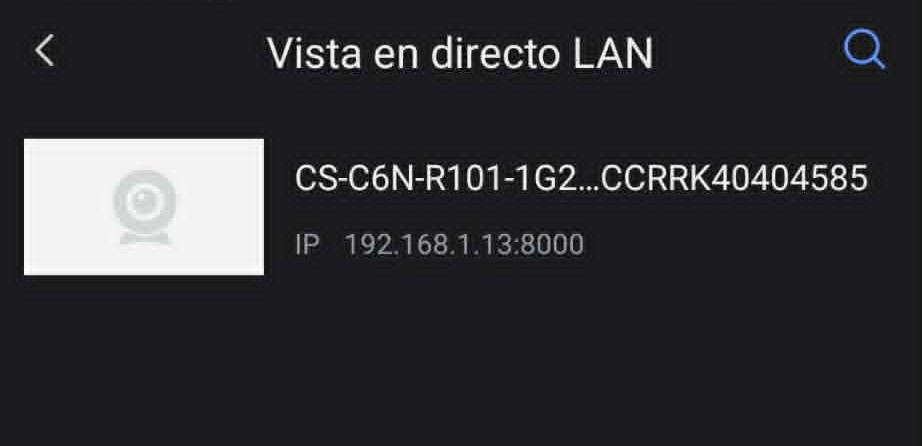
\includegraphics[width=0.5\linewidth]{ezviz_ip.jpeg}
    \caption{Ejemplo de búsqueda de IP de cámara EZVIZ. Cuenta > Ajustes > Vista en directo LAN. Nota: Ignorar el puerto.}
    \label{fig:rtsp_ezviz}
\end{figure}

\section{Detalles de funcionamiento}

\subsection{yolox}

Este paquete contiene toda la lógica y funciones para detectar objetos con un modelo YOLOX. Además contiene módulos para el entrenamiento de modelos con conjuntos de datos personalizados y para la ejecución de modelos con ONNX. Cuenta con una licencia Apache 2.0, por lo que puede ser modificado y distribuido.

El entorno de ejecución ONNX es un entorno optimizado para ejecutar modelos con un menor costo computacional y una mayor velocidad que con PyTorch. Los modelos ejecutados en este proyecto se ejecutan con ONNX, por lo que fue necesario usar el archivo \url{tools/export_onnx.py} para convertir los modelos de formato PyTorch (.pth) a formato ONNX (.onnx).

\begin{verbatim}
    python tools/export_onnx.py --output-name yolox_s.onnx -n yolox-s \
    -c yolox_s.pth
\end{verbatim}

Para entrenar el modelo de detección de armas se utilizó el script \url{tools/train.py}, el cual se configuró con el archivo de experimento \url{exps/example/yolo\_cctv\_weapon/yolo\_s\_weapon.py} con todos los parámetros de entrenamiento necesarios para el conjunto de datos Simuletic CCTV Weapon. Para más detalles de su uso, consultar la documentación del respositorio\footnote{\url{https://github.com/Megvii-BaseDetection/YOLOX/blob/main/docs/train_custom_data.md}}.

\begin{verbatim}
    python -m yolox.tools.train \
    -f exps/example/yolo_cctv_weapon/yolo_s_weapon.py \
    -d 1 -b 8 --fp16 -o
\end{verbatim}

Para ejecutar este comando se debe contar con un conjunto de datos de entrenamiento en formato COCO, el cual se puede generar con el script \url{scripts/format_cctv_weapon.py}, siempre y cuando se haya descargado el conjunto de datos Simuletic CCTV Weapon.

\begin{verbatim}
    python scripts/format_cctv_weapon.py "<PATH_DATASET>" "<PATH_OUTPUT>"
\end{verbatim}

Además, es necesario colocar el dataset generado en la carpeta \url{yolox/datasets/CCTV_Weapon} para que el script del experimento pueda encontrarlo.

\subsection{deepsort}

Este paquete cuenta con licencia MIT, lo que permitió hacer modificaciones para la adición de metadatos en las detecciones y las pistas de seguimiento, un nuevo estado, entre otros cambios menores y de compatibilidad.

El archivo principal de este paquete es \url{deepsort/tracker.py}, el cual contiene la clase DeepSortTracker que se encarga de toda la lógica del seguimiento de objetos.

\subsection{yoltracker}

Este paquete fue escrito desde cero y contiene la implementación de la detección de objetos, el seguimiento de objetos y el análisis de la escena. Está diseñado para ser importado como un paquete desde otros proyectos. Su archivo principal es \url{yolotracker/core.py} que contiene la clase YOLODetector, que corresponde al detector de objetos, y la clase YOLOEventDetector que realiza el seguimiento de objetos y el análisis de la escena.

Se incluyó el script \url{test_video.py} para probar el algoritmo desde videos pregrabados, con la intención de hacer modificaciones y evaluaciones de forma fácil, sin depender de una conexión con una cámara IP.

\begin{verbatim}
    python test_video.py --camera-id 1 --input-shape 640,640 \
    --file ../eval_dataset_cctv/events_videos/cctv_weapon_0001_weapon.mp4 \
    --model ../weights/yolox_s.onnx --onnx-provider cuda \
    --reid-model ../weights/osnet_x0_25.onnx --score-thr 0.5 \
    --weapon-model ../weights/yolox_s_weapon.onnx --weapon-score-thr 0.5 \
    --loitering-time=30 --object-time=15 --weapon-time=5 \
    --invasion-polygon="[[870, 275], [1600, 280], [1920, 810], [1920, 1080]]"
\end{verbatim}

Este script viene configurado con un detector de cada tipo de evento, las opciones --loitering-time, --object-time, --weapon-time e --invasion-polygon se utilizan para configurar los detectores.

Nota importante: Los tiempos de detección son segundos reales, no segundos del video, como se mencionó en una nota anterior.

\subsection{video-surveillance-app}

Esta es la carpeta de código de la aplicación. Contiene dos scripts principales, el archivo \url{wsgi.py} que se encarga de ejecutar el servidor web, y el archivo \url{scripts/tracking_service.py} que se encarga de iniciar el servicio de detección de los eventos en tiempo real.

\subsection{Soporte para múltiples cámaras}

En un flujo de datos simple, el procesamiento de los cuadros de video seguiría el ciclo siguiente: captura, procesamiento y nueva captura. Sin embargo, un sistema de videovigilancia implementado en un entorno real requiere el uso de más de una cámara de video a la vez, lo que implicaría crear un proceso diferente por cada cámara, multiplicando la cantidad de recursos de cómputo necesarios.

Una forma de evitar la duplicación de recursos es hacer que cada cámara capture y procese su video en un proceso/hilo independiente, pero todas las cámara utilicen los mismos modelos de detección de objetos y extracción de características. De esta forma, el sistema puede procesar videos de múltiples cámaras sin duplicar los modelos de detección de objetos y ahorrar espacio en memoria, sacrificando ligeramente el tiempo de detección. Esto es posible al emplear el paradigma de la programación concurrente descrito en la figura \ref{fig:video_capture}.

El flujo comienza con la creación de un hilo por cada cámara en el que se captura el video y se guardan los cuadros en una cola. Posteriormente, un hilo adicional mueve de forma constante el último cuadro capturado por cada cámara a una lista compartida de cuadros, es decir, una lista donde cada elemento contiene el último cuadro capturado por esa cámara. A continuación, se crea un subproceso que realiza la detección de objetos en cada cuadro de la cola compartida y coloca el resultado en otra lista compartida de colas de salida, es decir, una lista donde cada elemento es una cola con las cajas de detección, clases, etc. Finalmente, se crea un subproceso para cada cámara, en el que se realiza el seguimiento, se analian la escena y se detectan los eventos de seguridad.

Con esta configuración, se puede procesar el video proveniente de múltiples cámaras, sin la necesidad de aumentar el número de modelos que se deben cargar en memoria. El cuello de botella se presenta en el proceso que hace la detección de los objetos, sin embargo, en pruebas se detectó que el tiempo por cuadro solo aumenta de entre 0.1 a 0.16 segundos por cada cámara adicional.

\begin{figure}[h!]
    \centering
    \includegraphics[width=0.5\linewidth]{video_capture.pdf}
    \caption{Funcionamiento del módulo de captura de video e integración con otros módulos. Se muestran los nombres en inglés para mantener consistencia con la implementación.}
    \label{fig:video_capture}
\end{figure}


\section{Estrategia de entrenamiento}

Para la detección de armas de fuego se utilizó el modelo YOLOX\_s como base, preentrenado en el dataset COCO 2017 para detección de objetos. Se utilizó la técnica de transferencia de conocimiento sobre el modelo para que aprendiera a detectar dos clases: persona y arma.

La transferencia de conocimiento consiste en congelar todas las capas internas del modelo, o el backbone, reemplazar la capa de salida con una nueva y solamente entrenar esta capa de salida. En este caso, se sustituyó la capa de salida de 80 clases por una de 2 clases, y todos los demás pesos se congelaron.

El conjunto de datos de entrenamiento que se empleó fue el Simuletic Syntetic CCTV Weapon-Person dataset /CITE/, un conjunto de datos que contiene imágenes sintéticas de personas sosteniendo armas. Estas imágenes fueron generadas simulando que fueron capturadas por cámaras CCTV, lo que se alínea con el proyecto. En la figura \ref{fig:cctv_weapon_dataset} se muestran algunos ejemplos.

\begin{figure}[h!]
    \centering
    \includegraphics[width=0.8\linewidth]{cctv_weapon_dataset.pdf}
    \caption{Ejemplos de imágenes del conjunto de datos Simuletic Syntetic CCTV Weapon-Person.}
    \label{fig:cctv_weapon_dataset}
\end{figure}


El conjunto de datos contiene 141 imágenes a color con resoluciones variables y se separó un 80\% de los datos para entrenamiento y 20\% para validación. Además, se cuenta con un video de 6 segundos de duración para prueba.

Gracias a la facilidad de configuración de experimentos de la librería YOLOX los parámetros completos de entrenamiento pueden revisarse en el archivo \url{yolox/exps/example/yolox\_cctv\_weapon/yolox\_s\_weapon.py}. Estos parámetros se obtuvieron tras varios intentos y con configuraciones distintas, considerando las restricciones de hardware.

El entrenamiento se realizó en una computadora con Ubuntu 24.04.4 LTS, Intel Core i5-10300H, NVIDIA GeForce GTX 1050 Ti (4 GB), 8 GB RAM DDR4.

\section{Estrategia de evaluación}

La evaluación del sistema se realizará en tres partes: evaluación de la detección de objetos en imágenes, evaluación de detección de eventos en videos cortos y evaluación de detección de eventos en tiempo real con una cámara IP.

\subsection{Evaluación de detección de objetos}

Para la detección de objetos se emplearán las métricas mAP@0.5 y mAP@0.5:0.95. El mAP (mean Average Precision), o Precisión Media Promedio, es una métrica diseñada para evaluar la detección de objetos, considera no solo que la clase coincida, sino que también evalúa que el cuadro delimitador predicho coincida con el objetivo, utilizando el IoU (Intersection over Union).

El mAP@0.5 considera como una detección correcta cuando el IoU supera el 0.5, es decir, cuando más de la mitad del cuadro delimitador coincide con el cuadro objetivo. Por otra parte el mAP@0.5:0.95 calcula el promedio de los mAP con 10 umbrales de IoU (ej: 0.50, 0.55, 0.60, ..., 0.95) lo que lo hace más estricto.

El modelo YOLOX\_s preentrenado en COCO 2017 reporta un mAP@0.5:0.95 de \textit{40.5} para objetos de 80 clases, por lo que este es nuestro valor de referencia.

Debido a que el tipo de imagenes utilizadas en COCO 2017 (Figura \ref{fig:detection}) es diferente a lo que se esperaría obtener en un sistema de videovigilancia, se debe buscar un conjunto de datos apropiado para conocer el rendimiento real del sistema. Para ello se emplea el dataset VIRAT Ground Dataset 2.0 /CITE/\footnote{\url{https://viratdata.org/}}, el cual contiene videos de vigilancia de cámaras CCTV desde distintos ángulos y en distintos escenarios. Este conjunto de datos contiene anotaciones para las clases: persona, vehículo, bicicleta y bolsa, para cada cuadro de los videos. En la figura \ref{fig:virat_dataset} se muestran algunos ejemplos.

\begin{figure}[h!]
    \centering
    \includegraphics[width=0.9\linewidth]{virat_dataset.pdf}
    \caption{Ejemplos de cuadros de videos del conjunto de datos VIRAT Ground Dataset 2.0.}
    \label{fig:virat_dataset}
\end{figure}

Inicialmente se consideraron las 4 clases del modelo YOLOX\_s para evaluación, sin embargo, el dataset contiene muy pocas muestrs de los objetos de las clases vehículo ligero y bolsas. Además, con la estrategia alternativa de detección de objetos, ya no es necesario detectar estos objetos, por lo anterior solo se consideran 2 clases:

\begin{itemize}
    \item Persona
    \item Vehículo
\end{itemize}

Del conjunto de datos VIRAT Ground Dataset 2.0 se seleccionan 5 videos en escenarios distintos, de cada video se separan los cuadros del primer minuto del video para generar un conjunto de datos de evaluación.

En cuanto a la evaluación del modelo de detección de armas, se emplearán las mismas métricas, pero sobre el subconjunto de datos de validación del Simuletic Syntetic CCTV-Weapon dataset. Para este modelo, las dos clases a detectar son:

\begin{itemize}
    \item Persona
    \item Arma
\end{itemize}

\subsection{Evaluación de detección de eventos}

Para evaluar la detección de eventos se generan clips de longitud variable de algunos videos del dataset VIRAT. Además, se generaron algunos videos propios con una cámara de videovigilancia IP, como los que se muestran en la figura \ref{fig:custom_events}.

\begin{figure}[h!]
    \centering
    \includegraphics[width=0.9\linewidth]{custom_events.pdf}
    \caption{Ejemplos de videos capturados en cámara IP.}
    \label{fig:custom_events}
\end{figure}

En cada clip se presenta un tipo de evento, pudiendo presentarse el evento más de una ocasión. Por ejemplo, para el evento de merodeo, puede haber 3 personas merodeando en el mismo video, lo que daría un total de 3 eventos de merodeo por detectar. La evaluación consiste en comparar el número de eventos detectados por el sistema contra los presentes en el clip.

Las tablas \ref{tab:clips_merodeo}, \ref{tab:clips_intusion}, \ref{tab:clips_abandonado}, muestran un resumen de los videos que se emplearon para realizar la evaluación de los eventos de merodeo, intrusión y objeto abandonado, respectivamente.

\begin{table}
    \centering
    \begin{tabular}{llcc}
        \toprule
        Video          & Resolución & Duración      & N° Eventos  \\
        \midrule
        1              & 1920x1080  & 2:03          & 7           \\
        2              & 1920x1080  & 1:00          & 3           \\
        3              & 1280x720   & 0:30          & 5           \\
        \textbf{Total} &            & \textbf{3:33} & \textbf{15} \\
        \bottomrule
    \end{tabular}
    \caption{Clips de evaluación: \textbf{Merodeo}.}
    \label{tab:clips_merodeo}
\end{table}

\begin{table}
    \centering
    \begin{tabular}{llcc}
        \toprule
        Video          & Resolución & Duración      & N° Eventos \\
        \midrule
        1              & 1920x1080  & 0:10          & 4          \\
        2              & 1920x1080  & 0:13          & 2          \\
        3              & 1280x720   & 0:20          & 1          \\
        4              & 1820x1080  & 1:00          & 1          \\
        \textbf{Total} &            & \textbf{1:43} & \textbf{8} \\
        \bottomrule
    \end{tabular}
    \caption{Clips de evaluación: \textbf{Intrusión}.}
    \label{tab:clips_intrusion}
\end{table}

\begin{table}
    \centering
    \begin{tabular}{llcc}
        \toprule
        Video          & Resolución & Duración      & N° Eventos \\
        \midrule
        1              & 1920x1080  & 2:00          & 1          \\
        2              & 1920x1080  & 2:00          & 1          \\
        \textbf{Total} &            & \textbf{4:00} & \textbf{2} \\
        \bottomrule
    \end{tabular}
    \caption{Clips de evaluación: \textbf{Objeto abandonado}.}
    \label{tab:clips_abandonado}
\end{table}

Para la evaluación de la presencia de armas, solo se pudieron encontrar dos videos de grabaciones de cámaras CCTV, uno proveniente del conjunto de datos de entrenamiento, y otro de un conjunto de datos externo de cámaras infrarrojas, los cuales se muestran en la figura \ref{fig:weapon_dataset}. El resumen de sus características se muestra en la tabla \ref{tab:clips_arma}.

\begin{figure}[h!]
    \centering
    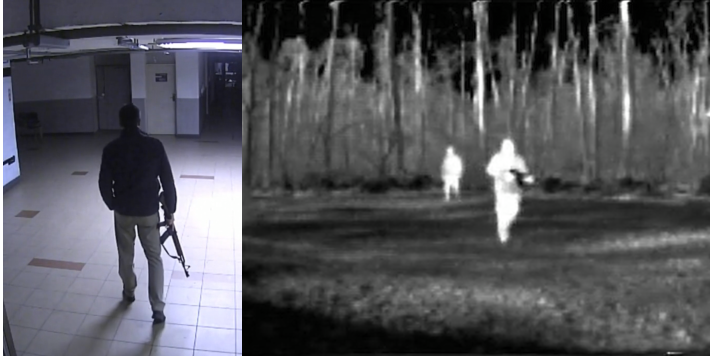
\includegraphics[width=0.4\linewidth]{weapon_dataset.pdf}
    \caption{Ejemplos de cuadros de videos de detección de armas.}
    \label{fig:weapon_dataset}
\end{figure}

\begin{table}
    \centering
    \begin{tabular}{llcc}
        \toprule
        Video          & Resolución & Duración      & N° Eventos \\
        \midrule
        1              & 464x688    & 0:06          & 1          \\
        2              & 320x240    & 0:10          & 1          \\
        \textbf{Total} &            & \textbf{0:16} & \textbf{2} \\
        \bottomrule
    \end{tabular}
    \caption{Clips de evaluación: \textbf{Arma}.}
    \label{tab:clips_arma}
\end{table}

\subsection{Evaluación en tiempo real}

Para la evaluación de detección en tiempo real se colocó una cámara IP en un área perimetral de una casa habitación. Esta cámara apunta hacia la calle y en ella se configuran eventos de intrusión, merodeo y abandono de objetos. En el video se presenta una persona que realiza la intrusión, merodeo y abandona un objeto, el sistema debe ser capáz de detectarlo.

Además de evaluar la detección de los eventos, se evaluarán métricas de rendimiento y velocidad de detección.

\section{Resultados}

\subsection{Detección de objetos}

En cuanto a la evaluación de la detección de objetos con YOLOX\_s, se obtuvieron un total de 1112 cuadros y 7376 objetos a detectar.

\begin{table}
    \centering
    \begin{tabular}{lcc}
        \toprule
        Clase          & AP@0.50      & N° Muestras \\
        \midrule
        Persona        & 0.23         & 4505        \\
        Vehículo       & 0.37         & 2841        \\
        \textbf{Media} & \textbf{0.3} &             \\
        \bottomrule
    \end{tabular}
    \caption{Evaluación de detección de objetos.}
\end{table}

En cuanto a la evaluación de la detección de armas con YOLOX\_s, se evaluaron un total de 141 imágenes y 282 objetos a detectar.

\begin{table}
    \centering
    \begin{tabular}{lcc}
        \toprule
        Clase          & AP@0.50      & N° Muestras \\
        \midrule
        Persona        & 0.43         & 141         \\
        Arma           & 0.17         & 141         \\
        \textbf{Media} & \textbf{0.3} &             \\
        \bottomrule
    \end{tabular}
    \caption{Evaluación de detección de armas.}
\end{table}

\subsection{Detección de eventos}

\begin{table}
    \centering
    \begin{tabular}{lccccc}
        \toprule
        Evento            & Accuracy     & Precision     & Recall        & F1            & FPS           \\
        \midrule
        Merodeo           & 0.84         & 0.95          & 0.88          & 0.90          & 8.6           \\
        Intrusión         & 0.86         & 0.86          & 1.00          & 0.91          & 6.5           \\
        Arma              & 0.50         & 0.50          & 0.50          & 0.50          & 10            \\
        Objeto Abandonado & 1.0          & 1.0           & 1.0           & 1.0           & 8             \\
        \textbf{Media}    & \textbf{0.8} & \textbf{0.82} & \textbf{0.84} & \textbf{0.82} & \textbf{8.27} \\
        \bottomrule
    \end{tabular}
    \caption{Evaluación de detección de eventos.}
\end{table}

\begin{table}
    \centering
    \begin{tabular}{lccccc}
        \toprule
            & Memoria (MiB) & Memoria GPU (MiB) & seg/cuadro & FPS \\
        \midrule
        GPU & 1223          & 376               & 0.198      & 5   \\
        CPU & 739           & 0                 & 0.357      & 2.8 \\
        \bottomrule
    \end{tabular}
    \caption{Evaluación de detección de eventos en videos.}
\end{table}

\subsection{Tiempo real}


\begin{table}
    \centering
    \begin{tabular}{lccc}
        \toprule
            & N° Cámaras & Memoria (MiB) & Memoria GPU (MiB) \\
        \midrule
        GPU & 1          & 2423          & 376               \\
        GPU & 2          & 2924          & 376               \\
        CPU & 1          & 2145          & 0                 \\
        CPU & 2          & 2778          & 0                 \\
        \bottomrule
    \end{tabular}
    \caption{Evaluación de detección de eventos en tiempo real.}
\end{table}

\begin{table}
    \centering
    \begin{tabular}{lcccc}
        \toprule
            & N° Cámaras & seg/captura & seg/procesamiento & seg/alarma  \\
        \midrule
        GPU & 1          & 0.076       & 0.102             & 0.109       \\
        GPU & 2          & 0.052/0.076 & 0.165             & 0.149/0.205 \\
        CPU & 1          & 0.063       & 0.332             & 0.384       \\
        CPU & 2          & 0.060/0.063 & 0.871             & 0.668/0.780 \\
        \bottomrule
    \end{tabular}
    \caption{Evaluación de detección de eventos en tiempo real.}
\end{table}

\section{Discusión}

\section{Conclusiones}

Summarize the work and propose future improvements or next steps.

% =================================================
\section*{Referencias}
\printbibliography

\end{document}